\subsection{Approval, Execution, and Evidence}
\label{sec:mech}

\begin{figure*}[t]
\centering
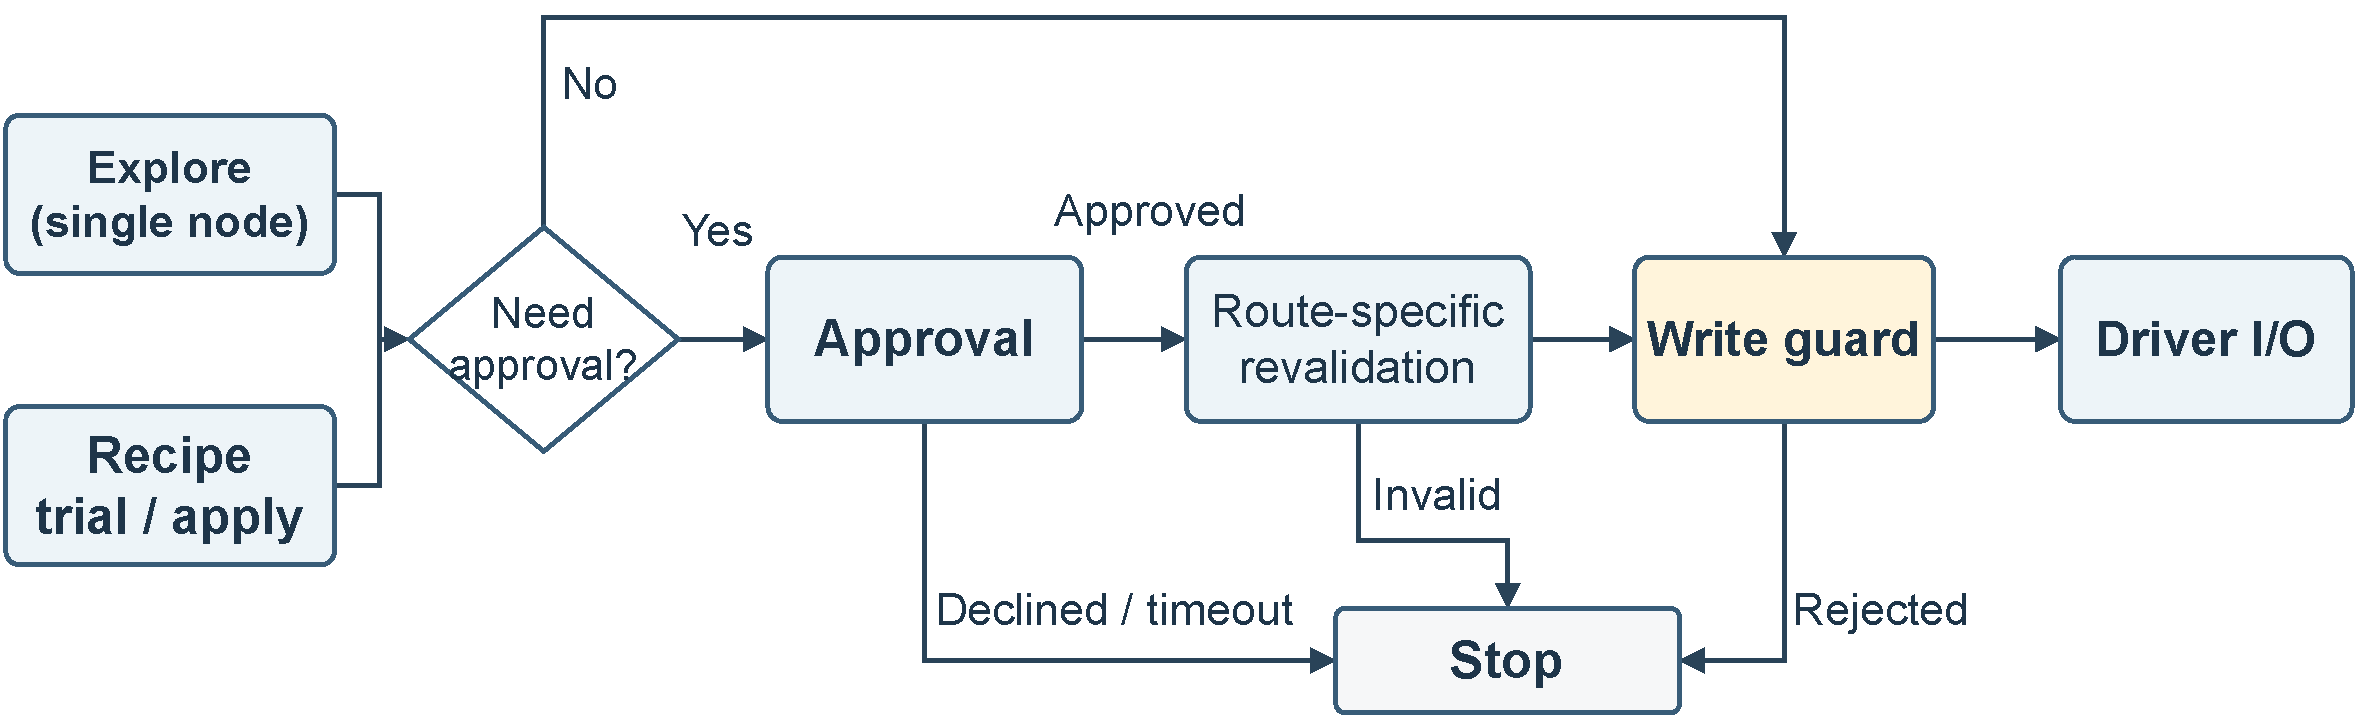
\includegraphics[width=\textwidth]{resources/fig4-governed-flow.pdf}
\caption{Simplified single-node \texttt{optimization\_explore} and recipe trial or apply write paths. Approved requests undergo route-specific revalidation. A decline, timeout, failed revalidation, or guard rejection stops the affected operation or parameter before driver dispatch. Other applicable dispatch and authorization checks are omitted; bypassing approval does not bypass them.}
\label{fig:hitl}
\end{figure*}
Fig.~\ref{fig:hitl} shows the conditional approval path and the bypass to the
shared write guard. For a manual single-node \texttt{optimization\_explore}
request, the approval service receives the node, proposed value, current
effective interval, and rationale. As in Algorithm~1, a decline or timeout
stops the request, while approval triggers revalidation of the original
direct node binding or the recipe binding and parameter membership. This path
does not use the recipe-operation context snapshot described below.
Revalidation does not make the checks and external device write atomic.

Recipe operations use a separate approval path. For \texttt{recipe\_trial}
and \texttt{recipe\_apply}, the approval is bound to the recipe operation and
active line--product--recipe--run context. After approval, the handler checks
authority and context again and verifies the recipe definition and
candidate scope before dispatch. A changed context, revoked binding, or
changed recipe definition prevents that proposal from proceeding. Recipe
trial approvals use a 30-minute window by default; single-node approval waits
expire after 180\,s by default. Outside benchmark mode, agent and manual
writes are subject to a minimum 60-s interval following a setpoint change;
recipe trials also use a per-line cadence of 300\,s by default.

A \texttt{recipe\_trial} submits a bounded batch through the configured
driver and returns a result for each parameter. Parameters are attempted
individually, so a batch can be partially applied; results and device state
must be reconciled before retrying. A trial does not save or apply a recipe
version. Before updating, applying, or rolling back the recipe, the caller can
retrieve later DAQ observations separately.

Receipts record the command outcome; observations record what followed in
the process. Command results are graded as readback-verified,
transport-acknowledged, or unverified. When a successful recipe write is not
already readback-verified, the service may, by default, attempt up to three additional
reads at 2\,s intervals where supported; recipe batches retain verification
outcomes for each parameter. A readback-verified result means that the
returned value matched the request within the applicable tolerance. A transport acknowledgement alone does not
establish that the device applied the value, and an unverified result does
not establish a matching readback. DAQ stores later timestamped process
observations, while recipe history, approvals, and task records remain with
their owning services. Identifiers and timestamps can link these records
when available, but a later observation alone does not prove that the command
caused the measured change. Section~\ref{sec:eval} evaluates selected parts
of this evidence chain under the stated test conditions.

